\documentclass{article}
\usepackage{fancyhdr}
\usepackage{amsmath,amssymb}
\usepackage{geometry}
\usepackage{datetime}
\usepackage{enumerate}
\usepackage{graphicx}

%Insert page formatting here
%\hoffset = -.5in
\voffset = -0.375in
%\textwidth = 6in
\textheight = 8in
\headheight = 24pt

\pagestyle{fancy}

\rhead{Peter Olson\\Student ID: $441666$}
\lhead{Math 3200\\Homework 5}
\chead{\today}
\cfoot{}

%\addtolength{\headwidth}{\marginparsep}
%\addtolength{\headwidth}{\marginparwidth}

%\renewcommand{\labelitemi}{$\diamond$}
\renewcommand{\implies}{\rightarrow}
\newcommand{\widespace}{\qquad \qquad \;}
\newcommand{\tret}{\\ \hline}
\newcommand{\fh}{\tfrac{1}{2}}
\newcommand{\deriv}[2]{\frac{d #1}{d #2}}
\newcommand{\pderiv}[2]{\frac{\delta #1}{\delta #2}}
\newcommand{\vr}{\vec{r}}
\newcommand{\at}{\text{ at }}
\newcommand{\var}{\text{Var}}

\begin{document}
\section*{Exercise 5.21}
\begin{enumerate}[\quad (a)]
	\item See R Code
	\item The resulting quantiles are very close to the Student-T distribution of $\chi^2_{4}$. $\chi^2_4$ has:
	
	
	25th Percentile: 1.9226
	
	50th Percentile: 3.357
	
	90th Percentile: 7.779
	\item See Plot
	\item The percentage probability that the ratio $> 4$, based on \texttt{show(mean(ratios > 4))}, is 0.09
	\item The sampling distribution of part (d) is $F_{4,4}$
	\item The sampling distribution of the inverse of part (d) is, likewise, $F_{4,4}$
\end{enumerate}
	\section*{Console Output}
	\begin{verbatim}
	> show(quantile(U_vec_1, c(.25, .5, .9)))
	25%      50%      90% 
	1.854227 3.263428 5.922892
	> show(mean(ratios > 4))
	[1] 0.09
	\end{verbatim}
	\section*{R Code}
	\begin{verbatim}
	n_1     <- 5
	mu_1    <- 10
	sigma_1 <- 3
	
	num_samples <- 100
	s_sq_1 <- vector()
	U_vec_1 <- vector()
	
	dist_matrix_1 <- matrix(nrow = 0, ncol = 5)
	
	# Part a
	
	for(i in 1:num_samples){
	dist_matrix_1 <- rbind(dist_matrix_1, rnorm(n_1, mu_1, sigma_1))
	}
	
	s_sq_1 <- apply(dist_matrix_1, 1, var)
	U_vec_1 <- (n_1 - 1) * s_sq_1 / (sigma_1^2)
	
	# Part b
	
	show(quantile(U_vec_1, c(.25, .5, .9)))
	
	# Part c
	
	n_2     <- 5
	mu_2    <- 5
	sigma_2 <- 3
	
	dist_matrix_2 <- matrix(nrow = 0, ncol = 5)
	
	for(i in 1:num_samples){
	dist_matrix_2 <- rbind(dist_matrix_2, rnorm(n_2, mu_2, sigma_2))
	}
	
	s_sq_2 <- apply(dist_matrix_2, 1, var)
	U_vec_2 <- (n_2 - 1) * s_sq_2 / (sigma_2^2)
	
	hist(U_vec_2, breaks=20)
	
	ratios <- (U_vec_1 / sigma_1^2) / (U_vec_2 / sigma_2^2)
	
	show(mean(ratios > 4))
	\end{verbatim}
	\section*{Plots}
	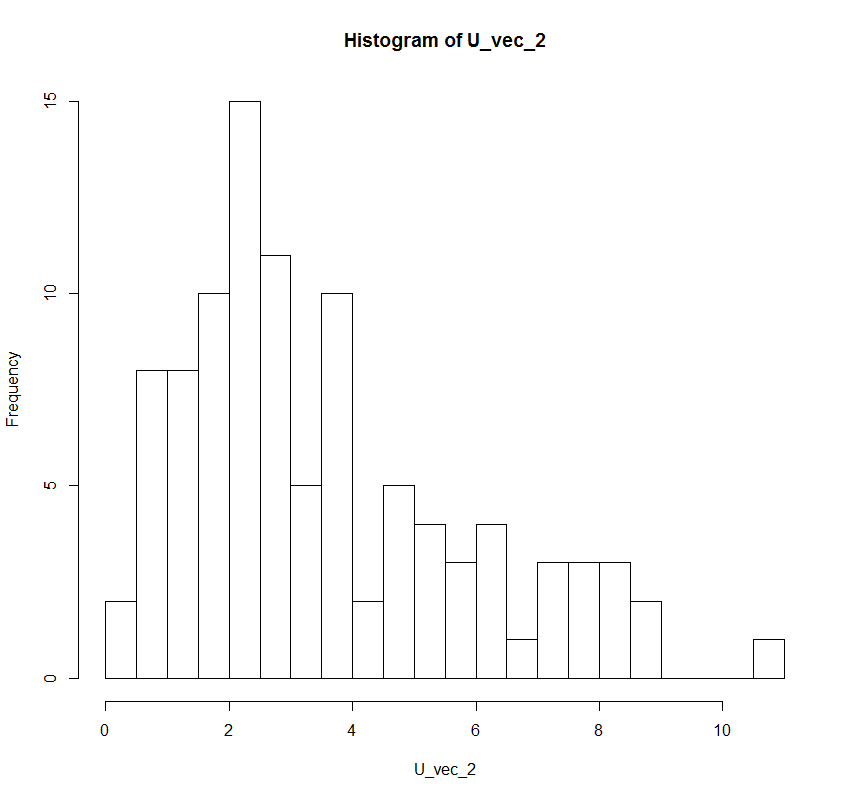
\includegraphics[width=4in]{q6}
\end{document}